\chapter{Kravspecifikation}

\begin{longtabu} to \linewidth{@{}l l l X[j]@{}}
    Version &    Dato &    Ansvarlig &    Beskrivelse\\[-1ex]
    \midrule
\label{version_Systemark}
\end{longtabu}


\section{Indledning}
Kravspecifikationen vil beskrive, ud fra en række modeller, hvordan blodtryksmåleren fungerer. Helt generelt er en invasiv blodtryksmåler et system, der vha. nål og tranducer kan måle 

\section{Ikke-funktionelle krav}
\subsection{(F)URPS+}
MoSCow er angivet i parentes ved hhv. M, S, C og/eller W, for Must, Should, Could og Won't\\


\textbf{Functionality}\\
(M) Brugeren skal kunne starte en ny måling indenfor XX sekunder efter opstart af programmet \\
(M) Systemet skal kunne kalibrere blodtrykssignalet\\
(M) Systemet skal kunne foretage en nulpunktsjustering\\
(M) Systemet skal kunne forstærke signalet fra transduceren (INDSÆT VÆRDI)\\
(M) Systemet skal kunne filtrere signalet med det indbyggede analoge antialiaserings filter med en båndbredde på 50 Hz \\
(M) Programmet skal kunne vise blodtrykket som funktion af tiden\\
(M) Programmet skal kunne vise blodtrykssignalet kontinuert\\
(M) Programmet skal programmeres i C\#\\
(M) Programmet skal kunne lagre de målte data i en database\\
(M) Programmet skal kunne filtrere blodtrykket via et digitalt filter\\
(S) Programmet bør kunne afbildede både systolisk og diastolisk blodtryk med tal\\
(S) Programmet bør kunne måle puls\\
(C) Programmet kan angive pulsslag med bip-lyde med varighed af 100ms og en frekvens på 850 Hz\\

\textbf{Usability}\\
(M) Blodtrykstallene der udskrives på brugergrænsefladen er røde\\
(S) Pulsmålingen skal udskrives på brugergrænsefladen med grønne tal\\
(M) Brugeren skal kunne starte en måling maksimalt 20 sekunder\\
Knapper??\\
Billede af brugergrænsefladen indsættes\\

\textbf{Reliability}\\
(M) Systemet skal kunne kører uden fejl i et år\\
(M) Systemet skal have en ”mean time to restore” på højest 24 timer\\
Systemet får herved en tilgænglighed beregnet ved \begin{align}
Availability = \frac{MTBF}{MTBF+MTTR} = \frac{365}{365+1} = 0,997 = 99,7 \%
\end{align}\\

\textbf{Performance}\\
(S) Systemet bør kunne gemme data på 5 sekunder +/-10%\\

\textbf{Supportability}\\
(M) Softwaren er opbygget af trelagsmodellen\\


\section{Funktionelle krav}
\subsection{Aktør-kontekst diagram}

\begin{figure}
	\centering
	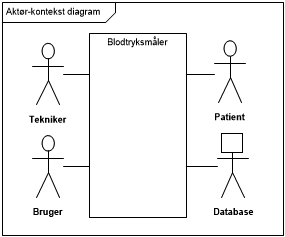
\includegraphics[width=0.6\textwidth]{Figurer/Aktordiagram}
\end{figure}

\subsection{Aktørbeskrivelse}
\begin{longtabu}to \linewidth{@{}l l X[j]@{}}
	{\large \textbf{Aktørnavn}} & {\large \textbf{Type}} & {\large \textbf{Beskrivelse}}\\ \toprule
	Bruger & Primær & Brugeren er den aktør der foretager blodtryksmålingerne. Brugeren er en person der har kendskab til systemet, samt tilladelse til at benytte systemet. Fx. sundhedsfaglig personale \\
	Tekniker & Primær & Tekniker er den aktør der foretager den årlige kalibrering af systemet. Teknikeren er en person der har kendskab til den tekniske del af systemet. Fx. medicotekniker på et sygehus\\
	Patient & Sekundær & Patienten stiller sin krop til rådighed for udførelse af en blodtryksmåling\\
	Database & Sekundær & Databasen er det sted, hvor blodtryksmålingens data gemmes
	
	
\end{longtabu}

\section{Use cases}
\subsection{Use case diagram}
\begin{figure}[H]
	\centering
	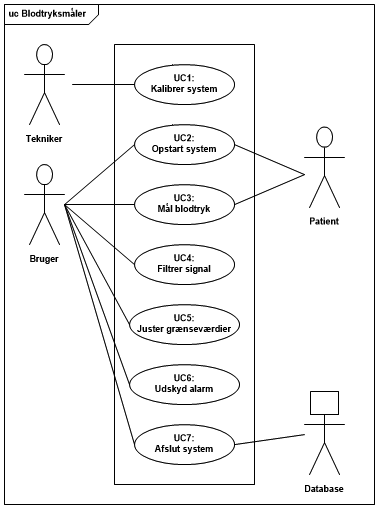
\includegraphics[width=0.7\textwidth]{Figurer/UCdiagram}
\end{figure}

\begin{longtabu} to \linewidth{@{}l r X[j]@{}} %UC1%
    {\large \textbf{Use Case 1}} && \\
    \toprule
    Navn &&    Kalibrer system\\
    Use case ID &&    1\\
    Samtidige forløb &&    1\\
    Primær aktør &&    Tekniker\\
    Initialisere &&    Tekniker ønsker at foretage kalibrering\\
    Forudsætninger &&  \\
    Resultat &&    Systemet er kalibreret                     \\ \midrule
    Hovedforløb &    1. &      \\ \midrule
                
    Undtagelser &    &    \\ \bottomrule
\caption{Fully dressed Use Case 1}
\label{UC1}
\end{longtabu}

\begin{longtabu} to \linewidth{@{}l r X[j]@{}} %UC2%
    {\large \textbf{Use Case 2}} && \\
    \toprule
    Navn &&    Opstart system\\
    Use case ID &&    2\\
    Samtidige forløb &&    1\\
    Primær aktør &&    Brugeren\\
    Initialisere &&    Brugeren ønsker at opstarte systemet\\
    Forudsætninger &&  Patienten er koblet korrekt til systemet jf. afledning I, samt use case 1 er gennemført.\\
    Resultat &&    Systemet er nulpunktsjusteret og brugeren er klar til at foretage en måling\\
    \midrule
    Hovedforløb &    1. &    Brugeren indtaster login-oplysninger og trykker på "Log-in"\--knappen \newline [1.a \textit{Forkert login}]\\
    	&			2. & Brugeren trykker på "nulstil"\--knappen. Systemet laver nulpunkts justering \newline [\textit{2.a Systemets nulpunktjustering er ikke korrekt}] \\ \midrule
    Undtagelser &    1a. & Besked om forkert login vises. Use Case fortsættes fra punkt 1     \\ 
    	&			2.a & Indikation om at systemet ikke er nulpunktjusteret vises. Use Case fortsættes fra punkt 2 \\ \bottomrule    
\caption{Fully dressed Use Case 2}
\label{UC2}
\end{longtabu}


\begin{longtabu} to \linewidth{@{}l r X[j]@{}} %UC3%
    {\large \textbf{Use Case 3}} && \\
    \toprule
    Navn &&    Mål blodtryk\\
    Use case ID &&    3\\
    Samtidige forløb &&    1\\
    Primær aktør &&    Brugeren\\
    Initialisere &&    Brugeren ønsker at foretage en blodtryksmåling\\
    Forudsætninger && UC2 er gennemført\\
    Resultat &&    At blodtrykket vises i kontinuerlig graf, systolisk og diastoliske blodtryk vises grafisk, samt puls vises grafisk                     \\ \midrule
    Hovedforløb &    1. &    Brugeren trykker på start måling\--kanppen\\
    			& 	 2. & Blodtrykgraf, systolisk, diastolisk og puls vises grafisk uden alarm\newline [2.a \textit{Blodtryk overholder ikke grænseværdier}] \\ \midrule               
    Undtagelser &    2.a & "Alarm" om at blodtryk er kritisk ift. de grænseværdier \\ \bottomrule
\caption{Fully dressed Use Case 3}
\label{UC3}
\end{longtabu}

\begin{longtabu} to \linewidth{@{}l r X[j]@{}} %UC4%
    {\large \textbf{Use Case 4}} && \\
    \toprule
    Navn &&    Filtrer signal\\
    Use case ID &&    4\\
    Samtidige forløb &&    2\\
    Primær aktør &&    Brugeren\\
    Initialisere &&    Brugeren ønsker at foretage en digital filtrering\\
    Forudsætninger && UC3 er igangsat\\
    Resultat &&    Det filtrerede signal vises i blodtryksgrafen                    \\ \midrule
    Hovedforløb &    1. &    Brugeren trykker på "filtrer signal"\--kanppen\\ \midrule               
    Undtagelser &    \\ \bottomrule
\caption{Fully dressed Use Case 4}
\label{UC4}
\end{longtabu}

\begin{longtabu} to \linewidth{@{}l r X[j]@{}} %UC5%
    {\large \textbf{Use Case 5}} && \\
    \toprule
    Navn &&    Juster grænseværdier\\
    Use case ID &&    5\\
    Samtidige forløb &&    2\\
    Primær aktør &&    Brugeren\\
    Initialisere &&    Brugeren ønsker at justere grænseværdierne for både systolisk og diastolisk blodtryk\\
    Forudsætninger && UC2 er gennemført\\
    Resultat &&    At grænseværdierne er sat efter patientens standarder                    \\ \midrule
    Hovedforløb &    1. &    Brugeren tilpasser diastoliske og systoliske grænseværdier\\ \midrule               
    Undtagelser &     &  \\  \bottomrule
\caption{Fully dressed Use Case 5}
\label{UC5}
\end{longtabu}


\begin{longtabu} to \linewidth{@{}l r X[j]@{}} %UC6%
    {\large \textbf{Use Case 6}} && \\
    \toprule
    Navn &&    Udskyd alarm\\
    Use case ID &&    6\\
    Samtidige forløb &&    2\\
    Primær aktør &&   Brugeren \\
    Initialisere &&    Brugeren ønsker at udskyde alarmen med ca. 60 sekunder \\
    Forudsætninger && UC3 er gennemført og undtagelse 2.a er igangsat\\
    Resultat &&    Alarmen er udskudt                  \\ \midrule
    Hovedforløb &    1. &    Brugeren trykker på "udskyd alarm"\--knap  \\ \midrule 		
    Undtagelser &     \\ \bottomrule
\caption{Fully dressed Use Case 6}
\label{UC6}
\end{longtabu}


\begin{longtabu} to \linewidth{@{}l r X[j]@{}} %UC7%
    {\large \textbf{Use Case 7}} && \\
    \toprule
    Navn &&    Afslut system\\
    Use case ID &&    7\\
    Samtidige forløb &&    1\\
    Primær aktør &&    Brugeren\\
    Initialisere &&    Brugeren ønsker at afslutte systemet og gemme måling\\
    Forudsætninger && UC3 er gennemført\\
    Resultat &&    Blodtryksmålingens data er gemt i database og bruger er logget ud af systemet                    \\ \midrule
    Hovedforløb &    1. &    Brugeren trykker på "afslut måling"\--knappen. "Gemme"\--vindue åbnes. \newline [1.a \textit{Bruger ønsker ikke atafslutte}]\\  						 	
                &    2. & Brugeren indtaster CPR-nr. \newline [2.a \textit{CPR-nr er ikke gyldigt}]	\\
                &    3. & Brugeren trykker på "gem og afslut"\--knappen. Systemet logger ud og afsluttes\\ \midrule                
    Undtagelser &    1.a. & Bruger trykker på "Annuller"\--knappen. Use Case 3 \\ 
    			&	2.a. &  Nyt CPR-nummer indtastet. Use Case fortsættes for punkt 2\\ \bottomrule
    		
\caption{Fully dressed Use Case 7}
\label{UC7}
\end{longtabu}





















